\chapter{THE INCIDENT RADIATION FIELD}
% !TEX root = hazy1.tex

\section{Overview}

The incident radiation field should be defined between the low-frequency limit
to the code, \emmmhz, corresponding to a wavelengths of \emmcm,
and the high-energy limit of \egamry, corresponding to an energy of \egamrymev.
The shape and its intensity or luminosity are usually specified
independently.
There are many ways to do this.

\section{The coarse and fine continua}

The code uses multi-grid methods to compute the overall spectral emission while
including  interactions among the
very large number of spectral lines (\citealp{Shaw2005}).  
The \cdTerm{coarse continuum} is used to define the
incident and diffuse continua.
A second \cdTerm{fine continuum} has much higher spectral resolving power and
is used to treat line transfer.
The fine continuum resolution is high enough to resolve overlapping spectral
lines.  
It is used to define line blocking coefficients that are passed up to the coarse continuum.  
This permits the effects of line overlap and velocity shear to be treated automatically.
The fine continuum does not include continuous
emission or absorption from the cloud so photoelectric or grain absorption will not be present
(this is treated in the coarse continuum).  
Only the very strongest absorption lines will be visible on the coarse continuum, but
the fine continuum will often show thousands of lines.
There are several options
on the \cdCommand{save continuum} command 
(page \pageref{sec:CommandSaveContinuum}) that report both of these continua
while various \cdCommand{set continuum} commands described on 
page \pageref{sec:CommandSetContinuumOptions} change details of this output.

Figure \ref{fig:CoarseFineContinua} compares parts of the fine (left panel) and
coarse (right panel) continua at a point near the H$^0$ - \htwo\ transition in 
the Orion H~II region / PDR.  
The fine continuum shows thousands of lines, mainly H~I and \htwo, but no emission.
The coarse continuum shows gas and dust emission and the effects of extinction of this emission.

\begin{figure}
\centering
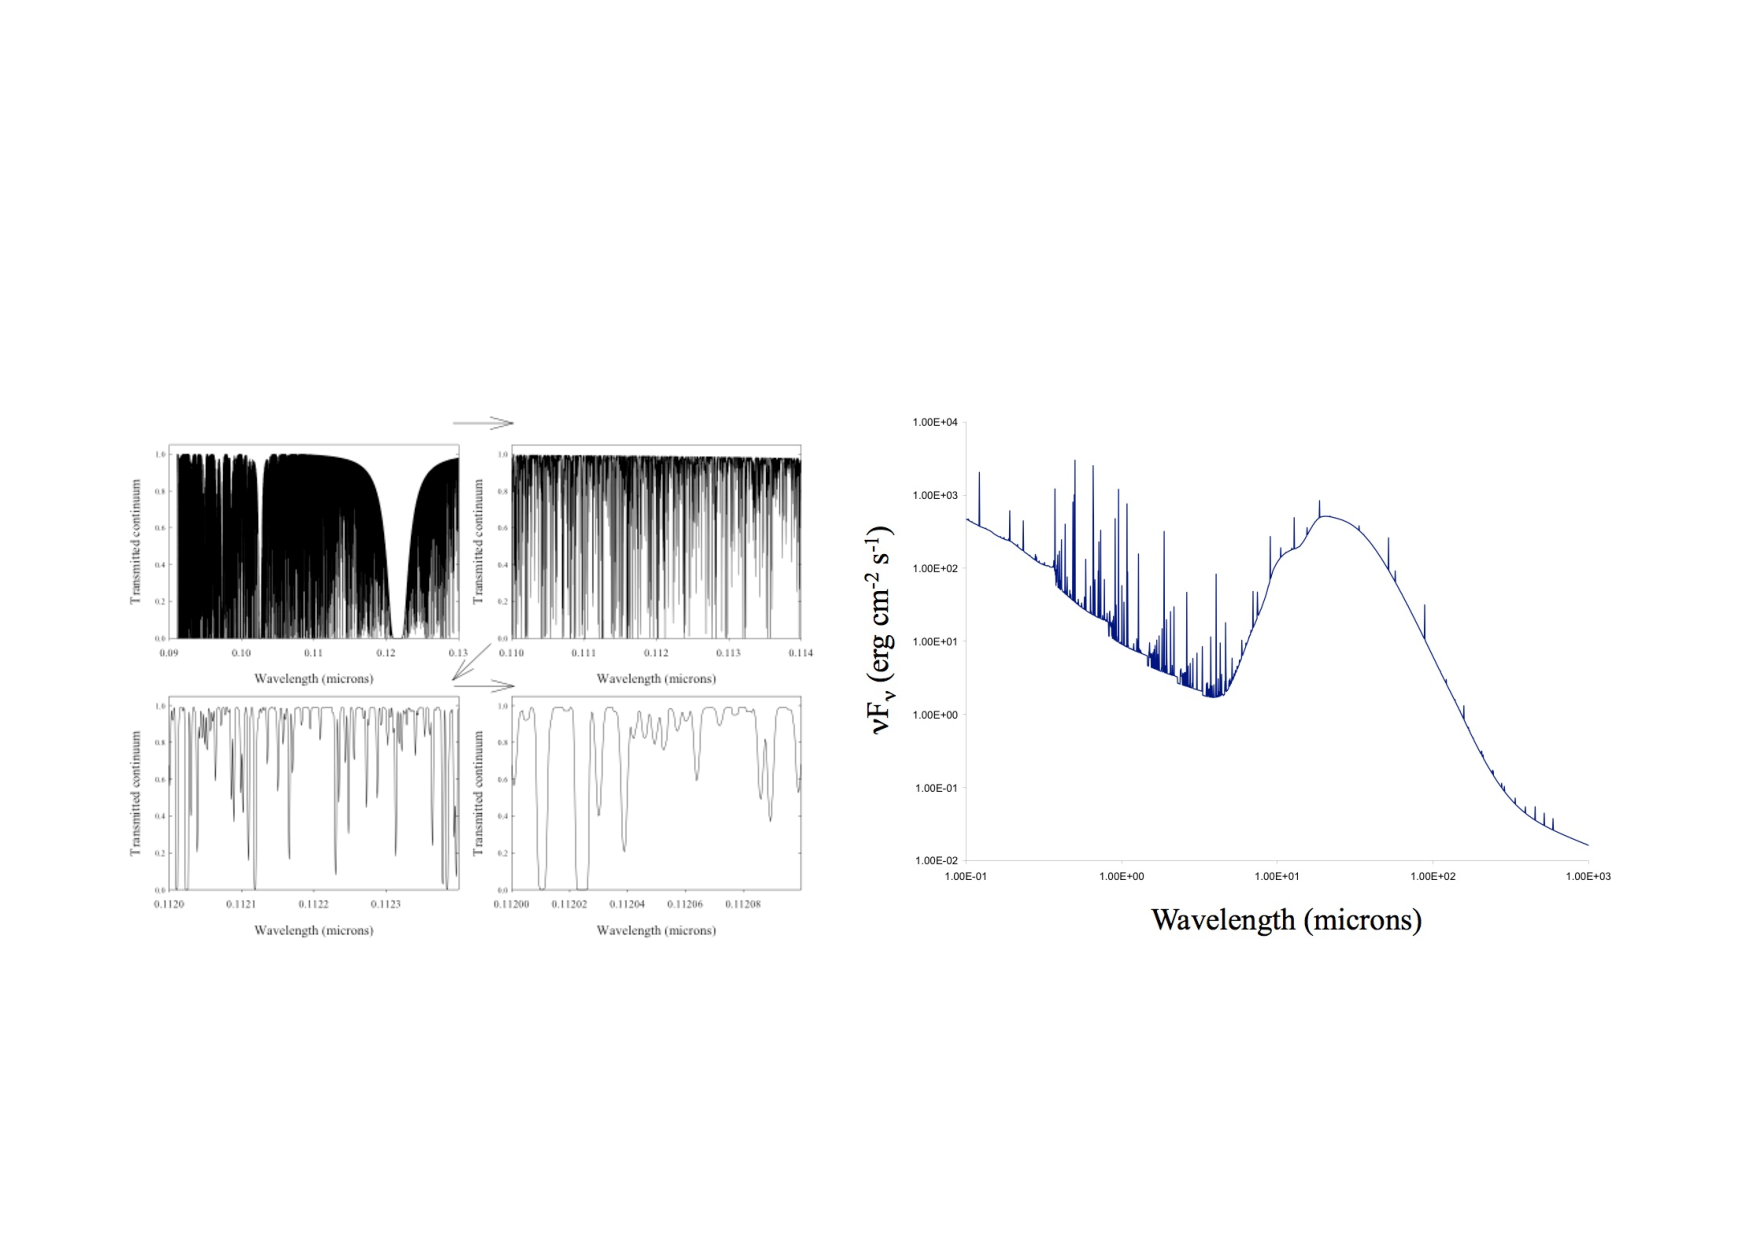
\includegraphics[scale=0.6]{CoarseFineContinua}
\caption[Orion Spectrum]{\label{fig:CoarseFineContinua}The spectrum of the Orion H~II region / PDR
at a point near the H$^0$ - \htwo\ transition.
The left panel shows the fine continuum and is taken from Figure 20 of \citet{Shaw2005}
It shows the extinction of the stellar SED by absorption lines formed in the gas.
The right panel shows the coarse continuum for a cloud stopping at this point and
mainly shows the extinguished stellar SEC also with dust and gas emission.}
\end{figure}

The spectral resolving power is defined as $E/\delta E$, where $E$ is the
photon energy and $\delta E$ the width of the resolution element.  The number
of energy bins needed to store the radiation field is proportional to the
resolving power.  The number of bins is a major pace setter for the code since it
must continuously reevaluate various integrals over the radiation field.
The resolving power of the
coarse continuum is defined in the file \cdFilename{continuum\_mesh.ini}
in the data directory.
This file is designed to be changed by the user and can be
changed to much higher resolving power if need be.  This is all described in
Section~\ref{Hazy2-sec:ChangingMeshResolution} in Part 2 of this document.
The resolution of the coarse continuum for a particular model can also be changed with the 
\cdCommand{set continuum resolution} command described on 
page \pageref{sec:CommandSetContinuumOptions}.
If you change the continuum resolution you will need to recompile
the stellar continuua and grain opacities so that their energy grid
agrees with that used by the code.

The resolving power of the fine continuum is established at the start of a calculation.
It needs to resolve lines, so the resolution depends on the lowest possible kinetic temperature
and any turbulence that may be present.
The \cdCommand{set fine continuum} command described on 
page \pageref{sec:CommandSetFineContinuum}
can also adjust this resolution.

\section{Defining a single component of the incident radiation field}

Two quantities, the \emph{shape} and \emph{intensity},
specify a single component of the incident radiation field.
The shape gives the form of the spectral energy distribution
but not its intensity.
The intensity can be specified as either the energy striking
the illuminated face of the cloud, referred to as
the intensity case, or both the source luminosity and the
distance separating the source and the cloud.  
The latter is referred to as the luminosity case.
The shape and intensity are specified independently
in most cases, although some commands specify both 
(the command specifying
the cosmic microwave background is an example of the latter).

In much of the following discussion we will refer to both
luminosity and intensity commands as simply intensity commands.
The distinction between the luminosity and intensity cases
is discussed further on page \pageref{sec:IntensityLuminosityCases}.

\section{Combining several radiation fields}

\subsection{The sum of several radiation fields}

It is possible to combine up to 100 incident radiation fields.\footnote{
Restrictions on the number of tables that could be entered existed
in \Cloudy\ versions 73 and before, but have been lifted. Restrictions on
which types of continua could be combined existed in \Cloudy\ versions 67
and before, but have been lifted.}   \Cloudy\ will stop if
more than 100 continua are entered.
This limit is set by the variable \cdVariable{LIMSPC}
that occurs in one of the included header files.

When more than one radiation field is entered the series of luminosity and
shape commands must be in the same order (i.e., map one to one).  There
must always be exactly the same number of luminosity and shape
specifications; \Cloudy\ will stop if there are not.

As an example, the following would be a rough approximation of an
accretion disk and boundary layer around a white dwarf:
\begin{verbatim}
# this is the black body associated with the boundary layer
# this is a shape command
black body, temperature =5e5 K
# this gives its total luminosity 
luminosity (total) 37.3
# the following shape is a rising power law, 
# a simple approximation to the disk 
power law, slope = 1.333, cutoff = 0.6 Ryd
# the total luminosity of this power law component
luminosity (total) 37.2
\end{verbatim}
The $5\times 10^5 \K$ blackbody has a total luminosity of
$10^{37.3} \ergps$ while
the power-law has a total luminosity of
$10^{37.2} \ergps $.

\subsection{Keeping shape and intensity commands together}

\noindent It is not absolutely necessary to keep
the ordered pairs of shape and
intensity commands together but this is a good practice
since some commands
(those given in Table \ref{tab:ShapeIntensityCommands})
specify \emph{both} the shape \emph{and} intensity of the incident
radiation field.
Problems arise if one of the commands giving both shape and intensity is
entered between another pair of shape and intensity commands.
For instance, the following will produce unintended results:
\begin{verbatim}
black body, temp = 5e5 K
CMB, z=2
luminosity (total) 37
\end{verbatim}
because the \cdCommand{CMB} command enters both the
shape and intensity of the cosmic microwave background.
In this example it comes after the \cdCommand{blackbody} command
specifies a shape, but before the \cdCommand{luminosity} command
specifies the luminosity of the blackbody.
As a result the intensity implicitly entered by the
\cdCommand{CMB}
command will apply to the hot blackbody rather than the cosmic
microwave background and the \cdCommand{luminosity} command will
then incorrectly set
the intensity of the cosmic background blackbody shape.
This problem cannot
occur if the shape and intensity commands are always kept together as in
the previous example.  The code should produce a warning if shape and
luminosity commands are mixed together with a command that enters both.

\begin{center}
\begin{table}
\centering
\caption{\label{tab:ShapeIntensityCommands}
Commands specifying both shape \emph{and} intensity}
\label{table:3}
\begin{tabular}{c}
\hline
background\\
 blackbody, energy density\\
blackbody, LTE\\
blackbody,
luminosity\\
blackbody, radius\\
CMB\\
table Draine\\
table HM96, HM05, HM12\\
table ISM\\
table read scale\\
\hline
\end{tabular}
\end{table}
\end{center}

\section{Check the incident radiation field!}

It is important to check that the incident radiation field
has been entered correctly.
First set up the commands to do a simulation and include the \cdCommand{save continuum} command
(described on page \pageref{sec:CommandSaveContinuum}).
Do the simulation and examine the
file produced by the \cdCommand{save continuum} command.
The first column gives the
photon energy and the second gives the incident radiation field
(as $\nu J_{\nu}$, erg cm$^{-2}$~s$^{-1}$)
at the illuminated face of the cloud.
Plot this radiation field and check that it is correct.

